\begin{flushleft}
Pour programmer la main il est indispensable d'avoir le logiciel Arduino IDE installé sur son ordinateur. Pour ce faire :\vspace{0.4cm}

\textbullet \, Se rendre sur le site : \url{https://www.arduino.cc/}\vspace{0.2cm}

\textbullet \, Aller sur \textit{SOFTWARE} et cliquer sur \textit{DOWNLOADS}

\begin{figure}[!h]
    \centering
    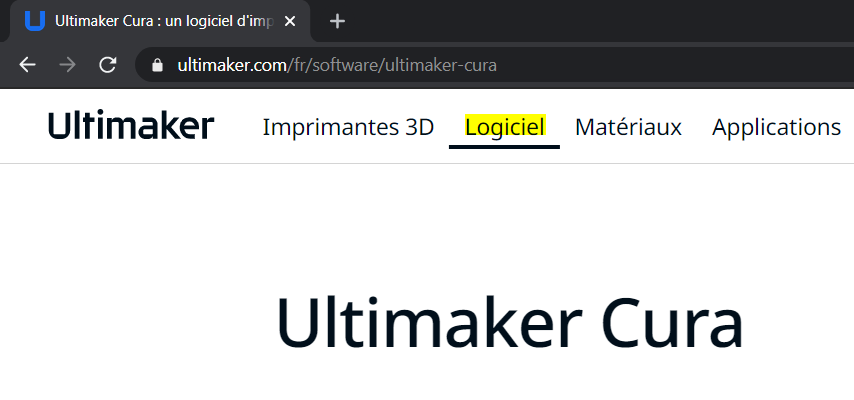
\includegraphics{Déroulé/Jour_3/Installation Arduino IDE/étape1.PNG}
    \caption{Installation Arduino IDE - \'Etape 1}
    \label{fig:my_label}
\end{figure}

%provisoire
\newpage

\textbullet \,  Sélectionner la version correspondant à votre ordinateur :
\begin{figure}[!h]
    \centering
    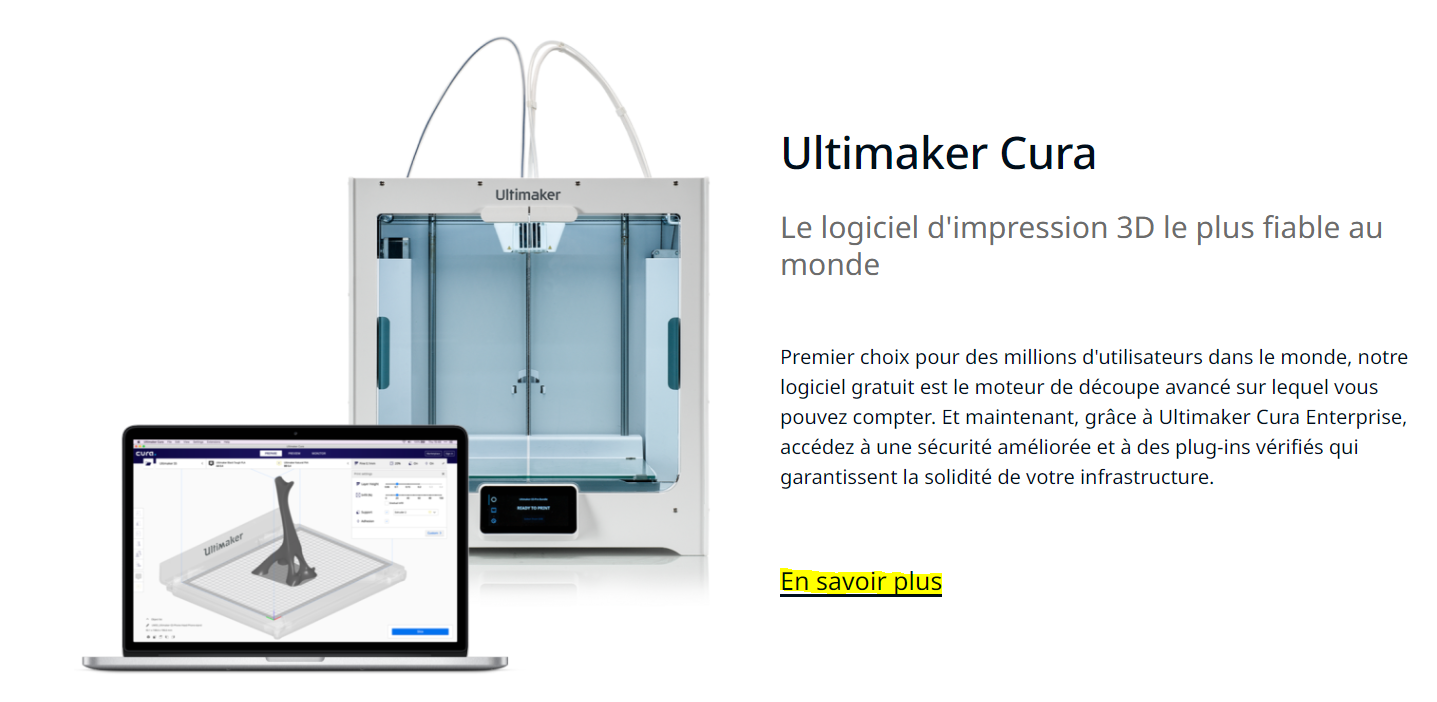
\includegraphics[width=450pt]{Déroulé/Jour_3/Installation Arduino IDE/étape2.PNG}
    \caption[\'Etape 2]{Installation Arduino IDE - \'Etape 2}
    \label{fig:my_label}
\end{figure}
\end{flushleft}